\documentclass[12pt]{amsart}

% PACKAGES ~~~~~~~~~~~~~~~~~~~

\usepackage{amsfonts, amsthm, amssymb, amsmath, stmaryrd, etoolbox, mathtools}
\usepackage[margin=1in]{geometry}
\usepackage{graphicx,caption,subcaption}
\usepackage{tikz}
\usetikzlibrary{matrix,arrows}

% NEW COMMANDS ~~~~~~~~~~~~~~~

% common math shorthands
\newcommand{\RR}{\mathbb{R}}
\newcommand{\ZZ}{\mathbb{Z}}
\newcommand{\NN}{\mathbb{N}}
\newcommand{\QQ}{\mathbb{Q}}
\newcommand{\CC}{\mathbb{C}}
\newcommand{\from}{\colon}
\newcommand{\xto}[1]{\xrightarrow{#1}}
\newcommand{\xgets}[1]{\xleftarrow{#1}}
\newcommand{\inv}{^{-1}}

% fonts
\newcommand{\cat}[1]{\mathbf{#1}}
\newcommand{\type}[1]{\mathtt{#1}}

% types
\newcommand{\tin}{\colon}
\newcommand{\A}{\type{A}}
\newcommand{\B}{\type{B}}
\newcommand{\C}{\type{C}}
\renewcommand{\P}{\type{P}}
\newcommand{\Q}{\type{Q}}
\newcommand{\BAC}{\B +_{\A} \C}
\newcommand{\Type}{\type{Type}}
\newcommand{\ap}{\type{ap}}
\newcommand{\inl}{\type{inl}}
\newcommand{\inr}{\type{inr}}
\newcommand{\glue}{\type{glue}}
\newcommand{\refl}{\type{refl}}
\newcommand{\code}{\type{code}}
\newcommand{\encode}{\type{encode}}
\newcommand{\decode}{\type{decode}}

% math operators
\DeclareMathOperator{\Hom}{Hom}
\DeclareMathOperator{\id}{id}
\DeclareMathOperator{\ob}{Ob}
\DeclareMathOperator{\arr}{arr}
\DeclareMathOperator{\im}{im}
\DeclareMathOperator{\Aut}{Aut}
\DeclareMathOperator{\Bij}{Bij}
\DeclareMathOperator{\Sub}{Sub}

% theorem styles
\newtheorem{lemma}{Lemma}
\newtheorem{thm}{Theorem}
\newtheorem{prop}{Proposition}
\newtheorem{cor}{Corollary}
\theoremstyle{remark}
\newtheorem{rmk}{Remark}
\theoremstyle{definition}
\newtheorem{defn}{Definition}
\newtheorem{ex}{Example}

% editing
\newcommand{\daniel}[1]{{\color{red} \textbf{DANIEL}: #1 }}
\newcommand{\amelia}[1]{{\color{green} \textbf{AMELIA}: #1 }}
\newcommand{\chandrika}[1]{{\color{blue} \textbf{CHANDRIKA}: #1 }}

%%%%%%%%%%%%%%%%
% begin document
%%%%%%%%%%%%%%%%

\begin{document}
\title{A pushout of sets over an injection is a set}
\maketitle

\section{The 'pushout is a set' theorem presented} %~~~~~~~~~~~~~~~

\begin{thm} \label{thm:pushout-is-set}
  Given mere sets \( \A \), \( \B \), and \( \C \) configured in a
  span
  \[
    \C \xgets{g} \A \xto{f} \B
  \]
  where \( f \) is monic, then the pushout \( \BAC \) is a mere set.
\end{thm}

\daniel{In the following paragraph, we define $ \P $ which encodes
  those id-types of $ \BAC $ that are propositions. The pushout
  $ \BAC $ is a set when $ \P $ contains all id-types in the
  pushout. So we define $ \Q $ to encode all id-types of $ \BAC $,
  which means that showing that $ \BAC $ is a set is the same as
  showing that $ \Q $ is equivalent to $ \P $. }

Denote the canonical pushout maps as \( \inl \from \B \to \BAC \) and
\( \inr \from \C \to \BAC.  \) Consider the types
\[
  \P \coloneqq
  \{ (x,y) \tin ( \BAC ) \times ( \BAC ) \vert
  x =_{\BAC} y \text{ is a mere proposition} \}
\]
and 
\[
  \Q \coloneqq (\BAC) \times (\BAC).
\]
To prove the theorem, it is sufficient to show that the inclusion
\(
  \P \hookrightarrow \Q
\)
is an equivalence. 

% ~~~~~~~~~~~~~~~~~~~

\begin{lemma} \label{thm:inclusion-is-embedding}
  The inclusion
  \(
    \P \to \Q
  \)
  is an embedding.
\end{lemma}

\begin{proof}
  We need to show that, for each
  \(
     ( x_0 , y_0 ) \tin \Q,
  \)
  the homotopy fibre
  \[
     \type{F} \coloneqq
     \sum\limits_{ ( x,y ) \tin \P}
     ( x,y ) =_{\Q} ( x_0,y_0 )
  \]
  is a mere proposition. Any
  \(
    p \tin \type{F},
  \)
  is a pair of paths
  \(
    p_x \tin x =_{\BAC} x_0
  \)
  and
  \(
    p_y \tin y =_{\BAC} y_0.
  \)
  The existance of such a $p$ implies that 
  \(
    ( x_0,y_0 ) \tin \P
  \)
  by $ \beta $-reducing $ (x,y) $ to $ ( x_0,y_0 ) $. Therefore,
  \(
    \refl_{ ( x_0,y_0 ) } \tin \type{F}.
  \)
  The cube of paths
    \[
      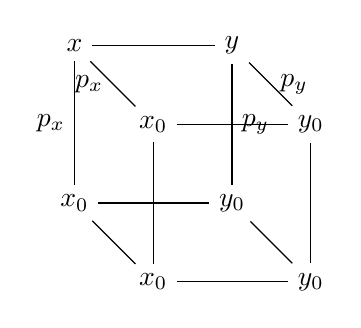
\begin{tikzpicture}
        \node (1) at (0,2) {\( x \)};
        \node (2) at (2,2) {\( y \)};
        \node (3) at (1,1) {\( x_0 \)};
        \node (4) at (3,1) {\( y_0 \)};
        \node (5) at (0,0) {\( x_0 \)};
        \node (6) at (2,0) {\( y_0 \)};
        \node (7) at (1,-1) {\( x_0 \)};
        \node (8) at (3,-1) {\( y_0 \)};
        \draw [-] (1) to (2);
        \draw [-] (3) to (4);
        \draw [-] (5) to (6);
        \draw [-] (7) to (8);
        \draw [-] (1) to node [left] {\( p_x \)} (3);
        \draw [-] (2) to node [right] {\( p_y \)} (4);
        \draw [-] (5) to (7);
        \draw [-] (6) to (8);
        \draw [-] (1) to node [left] {\( p_x \)} (5);
        \draw [-] (2) to node [right] {\( p_y \)} (6);
        \draw [-] (3) to (7);
        \draw [-] (4) to (8); 
      \end{tikzpicture}
    \]
    commutes trivially and is filled because \( \BAC \) is at most a
    1-type. Hence, we have that
    \(
       p =_{ \type{F} } \refl_{ ( x_0,y_0 ) }
    \)
    and \( \type{F} \) is contractible.

    \daniel{Where do we use that 'being a proposition' is a
      proposition?}
\end{proof}

% ~~~~~~~~~~~~~~~~~~~

To prove that
\( 
   \P \hookrightarrow \Q
\)
is an equivalnece, it remains to show that \( \P \) contains a point
in every connected component of \( \Q \). Note that every connected
component of \( \BAC \) contains a point of form \( \inl b \) or
\( \inr c \). Therefore, if
\(
   \inl b =_{\BAC} x
\)
and
\(
   \inr c =_{\BAC} x
\)
are always mere propositions, then \( \P \) contains a point in every
component of \( \Q \) as desired.

To actually do this, we employ the \textit{encode-decode method}. The
strategy is to introduce types
\[
   \prod\limits_{ x \tin \BAC} \code ( \inl b , x )
   \textrm{ and }
   \prod\limits_{ x \tin \BAC } \code ( \inl c , x ).
\]
After showing these are mere propositions---an easier task than
proving the identity types in \( \BAC \) are mere propositions---we build
an equivalence between
\[
  \prod\limits_{ x \tin \BAC } \code ( \inl b , x )
  \textrm{ and }
  \prod\limits_{ x \tin \BAC } \inl b =_{\BAC} x,
\]
and likewise between
\[
  \prod\limits_{ x \tin \BAC } \code ( \inr c , x )
  \textrm{ and }
  \prod\limits_{ x \tin \BAC } \inr c =_{\BAC} x.
\]

% ~~~~~~~~~~~~~~~~~~~~~
% ~~~~~~~~~~~~~~~~~~~~~

\subsection{Defining \( \prod\limits_{x \tin \BAC} \code ( \inl b , x ) \)} 
\label{sec:define-code-bx}

To define
\[
  \prod\limits_{ x \tin \BAC } \code ( \inl b , x ),
\]
we use structural induction on \( x \). Thus we compute the values
\begin{itemize}
\item \( \code ( \inl b ,\inl b' ) \),
\item \( \code ( \inl b , \inr c ) \), and
\item \( \code ( \inl b , \glue a ) \).
\end{itemize}
We also show that the first two are mere propositions.  

Define
\(
    \code ( \inl b , \inl b' )
\)
as the pushout of the span
\[
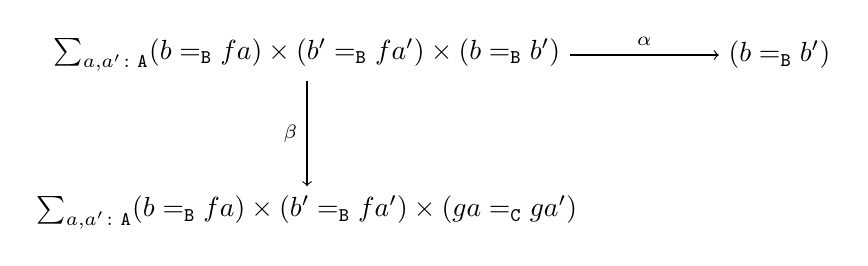
\begin{tikzpicture}
	\node (1) at (0,2) 
		{ $ \sum_{ a , a' \tin \A } 
			( b =_\B fa ) 
			\times ( b' =_\B fa' ) 
			\times ( b =_\B b' ) $ };
	\node (2) at (6,2) 
		{ $ ( b =_\B b' ) $ };
	\node (3) at (0,0) 
		{ $ \sum_{ a , a' \tin \A } 
			( b =_\B fa ) 
			\times  (b' =_\B fa') 
			\times ( ga =_\C ga' ) $ };
	\draw [ -> ] (1) to 
		node [above] {\scriptsize $ \alpha $} 
		(2);
	\draw [ -> ] (1) to 
		node [left] {\scriptsize $ \beta $}
		(3);
\end{tikzpicture}
\quad 
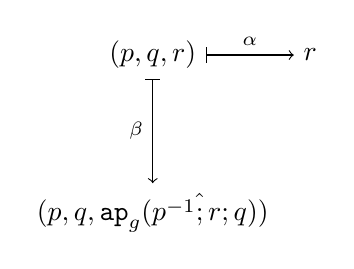
\begin{tikzpicture}
	\node (1) at (0,2) { \( ( p,q,r )  \) };
	\node (2) at (2,2) { \( r \) };
	\node (3) at (0,0) { \( ( p,q, \ap_g (\hat{p\inv ; r ; q})) \)};
        \draw [ |-> ]
          (1) to 
	  node [above] {\scriptsize $ \alpha $} 
	  (2);
        \draw [ |-> ]
          (1) to 
	  node [left] {\scriptsize $ \beta $}
	  (3);
\end{tikzpicture}
\]
where
\(
    \hat{p\inv ; r ; q}
\)
is the preimage of the path
\(
    p\inv ; r ; q \tin
    fa =_{\B} fa'
\)
Its existance and uniqueness follows from
the injectivity of \( f \).

To distinguish these pushout maps from those associated to \( \BAC \),
we denote them by \( \inl' \) and \( \inr' \).

In the following lemma, we use the denotation
\(
    \type{X} \coloneqq
    \sum_{ a , a' : \A }
    ( b =_\B fa ) \times ( b' =_\B fa') \times ( ga =_\C ga' ),
\)
\(
    \type{Y} \coloneqq
    \sum_{ a , a' : \A }
    ( b =_\B fa ) \times ( b' =_\B fa' ) \times ( b =_/B b' ),
\)
and
\(
    \type{Z} \coloneqq b =_\B b'.
\)

% ~~~~~~~~~~~~~~~~~~~

\begin{lemma} \label{thm:code-bb-isProp}
  The type
  \(
      \code ( \inl b , \inl b' )
  \)
  is a mere proposition.  
\end{lemma}
\begin{proof}
  The feet of the span are mere propositions; \( \type{Z} \) trivially
  so. Showing that \( \type{X} \) is also a mere proposition requires
  some work. Pick
  \(
      ( r,s,t ) \tin
      ( b =_\B fa ) \times ( b' =_\B fa') \times ( ga =_\C ga' )
  \)
  and
  \(
      ( r',s',t' ) \tin
      ( b =_\B fa'' ) \times ( b' =_\B fa''') \times ( ga'' =_\C ga'''').
  \)
  Then
  \(
      r\inv ; r' \tin fa =_\B fa''
  \)
  and
  \(
      s\inv ; s' \tin fa' =_\B fa''',
  \)
  along with the injectivity of \( f \), ensure the existance of paths
  \(
      \hat{r} \tin a =_\A a''
  \)
  and
  \(
      \hat{s} \tin a' =_\A a'''.
  \)
  Beta-reduction provides that
  \(
      ( b =_\B fa ) \times ( b' =_\B fa') \times ( ga =_\C ga' )
  \)
  is equivalent to
  \(
     ( b =_\B fa'' ) \times ( b' =_\B fa''') \times ( ga'' =_\C ga'''' ),
  \)
  both of which are contractable because \( \B \) and \( \C \)
  are mere sets.  It follows that
  \(
      ( r,s,t ) = ( r',s',t' ).
  \)

  If
  \(
      \code ( \inl b , \inl b' )
  \)
  is not empty, then one of the span's feet must also be
  non-empty.  This leads to three cases:
  \begin{itemize}
  \item
    \( \type{X} \) is empty and \( \type{Z} \) is non-empty. This
    forces \( \type{Y} \) to also be empty and so the lemma holds;
  \item
    \( \type{X} \) is non-empty and \( \type(Z) \) is empty. This
    again forces \( \type{Y} \) to be empty, so the lemma holds;
  \item
    \( \type{X} \) and \( \type{Z} \) are non-empty. It is quick to check
    that this forces \( \type{Y} \) to be non-empty. We dedicate the
    remainder of this proof to showing \( \code ( \inl b , \inl b' )
    \) is a proposition in this case.
  \end{itemize}
  
  A point in the apex of the span provides a witness to
  \(
      fa =_\B fa'
  \)
  which in turn provides a witness to
  \(
      a =_\A a'.
  \)
  Beta-reduction plus univalence equates
  \[
    \type{Y} =
    \sum\limits_{a \tin \A}
    (b=_{\B} fa) \times (b'=_{\B} fa) \times (b=_{\B} b')
  \]
  and also
  \[
    \type{X} =
    \sum\limits_{a \tin \A}
    (b=_{\B} fa) \times (b'=_{\B} fa) \times ( ga =_{\C} ga )
  \]
  The third terms of each of these types are redudant because \( \B \)
  and \( \C \) are mere sets. Applying beta-reduction and univalence
  again equates
  \[
    \type{Y} =
    \sum\limits_{a \tin \A}
    (b=_{\B} fa) \times (b'=_{\B} fa)
  \]
  and
  \[
    \type{X} =
    \sum\limits_{a \tin \A}
    (b=_{\B} fa) \times (b'=_{\B} fa),
  \]
  hence
  \(
      \type{X} = \type{Y}.
  \)
  It follows that
  \(
      \code ( \inl b , \inl b')
  \)
  is equivalent to the pushout of the span
  \[
    \begin{tikzpicture}
      \node (1) at (-1,1) {\( \type{X} \)};
      \node (2) at (-1,-1) {\( \type{X} \)};
      \node (3) at (1,1) {\( \type{1} \)};
      \draw [->] (1) to node [left] {\( \id \)} (2);
      \draw [->] (1) to node [above] {\( ! \)} (3);
    \end{tikzpicture}
  \]
  which is a mere set.
\end{proof}

% ~~~~~~~~~~~~~~~~~~~~~~~~~~~~~~

This completes our current work with
\(
    \code ( \inl b , \inl b' ).
\)

Next, define
\[
  \code ( \inl b , \inr c ) \coloneqq
  \sum_{ a : \A } ( b =_\B fa ) \times ( c =_\C ga ).
\]

\begin{prop}
  $ \code ( \inl b , \inr c ) $ is a mere proposition.
\end{prop}


\begin{proof}
  Indeed, if there does not exist an $ a : A $ such that
  $ b =_B f ( a )$ and $ c' =_C g ( a ) $ are both populated, then
  $ \type{ code } \left( \inl( b ) , \inr( c' ) \right) $ is empty.
  If there exists a single $a : A$ such that $ b =_B f ( a )$ and
  $ c' =_C g ( a ) $ are both populated, then because they are each
  equivalent to $ \type{ 1 }$,
  $ \type{ code } \left( \inl( b ) , \inr( c' ) \right) $ is also
  equivalent to $ \type{ 1 }$.  If there is $a, a' : A$ such that
  $ b =_B f ( a )$ and $ c' =_C g ( a ) $, and also $ b =_B f ( a' )$
  and $ c' =_C g ( a' ) $, then the injectivity of $f$ and
  $f ( a ) =_B b =_B f ( a' )$ implies that $a =_A a'$ which also
  gives us that
  $ \type{ code } \left( \inl( b ) , \inr( c' ) \right) $ is
  equivalent to $ \type{ 1 }$.
\end{proof}

Finally, we need to construct a witness to
\[
  \code ( \inl b , \ap_{\glue} a ) \tin
  \code ( \inl b , \inl fa ) =
  \code ( \inl b , \inr ga ). 
\]
Because both sides of the equation are mere propositions, it suffices
to show that they are simultaneously empty or populated.

% ~~~~~~~~~~~~~~~~~~~~~~~~~~~~~~

\begin{lemma} \label{thm:code-faga-populated-empty}
  There exist functions
  \(
      \code ( \inl b , \inl fa ) \to \code ( \inl b , \inr ga )
  \)
  and
  \(
      \code ( \inl b , \inl fa ) \to \code ( \inl b , \inr ga ).
  \)
  Moreover, they form an equivalence.
\end{lemma}
\begin{proof}
  Suppose
  \(
      \code ( \inl b , \inl ga )
  \)
  is inhabited. This point is equal 
  \(
      ( p , \refl_{ga} )
  \)
  and \( p \) is pushed forward to populate
  \(
      \code ( \inl b , \inl fa ). 
  \)
  
  suppose that
  \(
       \code ( \inl b , \inl fa )
  \)
  is inhabited. This implies that either
  \(
       p \tin b =_{\B} fa 
  \)
  or
  \(
     ( q,r,s ) \tin
     ( b =_{\B} fa' ) \times ( fa =_{\B} fa'' ) \times ( ga' =_{\C} ga'' )
  \)
  in the first case,
  \(
      ( p , \refl_{ga} ) \tin \code ( \inl b , \inr ga )
  \)
  in the second case, the injectivity of \( f \) allows us to
  beta-reduce \( a \) to \( a'' \). That is, we actually have that
  \(
      (q,r,s) \tin
      ( b =_{\B} fa' ) \times ( fa =_{\B} fa ) \times ( ga' =_{\C} ga )
  \)
  hence
  \(
      ( q , s\inv ) \tin \code ( \inl b , \inr ga ).
  \)

  the functions form an equivalence because both
  \(
      \code ( \inl b , \inl fa )
  \)
  and
  \(
      \code ( \inl b , \inr ga )
  \)
  are propositions.
\end{proof}

% ~~~~~~~~~~~~~~~~~~~~~~~~
% ~~~~~~~~~~~~~~~~~~~~~~~~

\subsection{Define \( \prod_{x \tin \BAC } \code ( \inr c , x ) \)} 
\label{sec:codecx}

To define
\(
    \prod\limits_{x \tin \BAC} \code ( \inr c , x  )
\)
requires us to compute three values:
\begin{itemize}
\item \( \code ( \inr c , \inl b ) \),
\item \( \code ( \inr c , \inr c' ) \), and
\item \( \code ( \inr c , \glue a ) \),
\end{itemize}
the first two of which we show are mere propositions.

Define
\[
  \code ( \inr c , \inl b ) \coloneqq
  \sum_{ a : \A } ( c =_\C ga ) \times ( b =_\B fa ).
\]

\begin{lemma} \label{thm:code-cb-isprop}
  The type \( \code ( \inr c , \inl b ) \) is a proposition.
\end{lemma}
\begin{proof}
  See lemma~\ref{thm:code-cb-isprop}.   
\end{proof}

Define
\[
  \code ( \inr c , \inr c' ) \coloneqq \sum_{ a , a' : a }
  ( c =_\C ga ) \times ( c' =_\C ga' ) \times ( fa =_\B fa' ).
\]

\begin{lemma} \label{sec:code-cc-isprop}
  The type \( \code ( \inr c , \inr c' ) \) is a mere proposition.
\end{lemma}
\begin{proof}
  Because \( f \) is in injection, \( a =_\A a' \) is populated so
  \(
      \code ( \inr c , \inr c' )
  \)
  beta-reduces to
  \[
    \sum\limits_{a,a' \tin \A}
    ( c =_\C ga ) \times ( c' =_\C ga ) \times ( a =_\A a )
  \]
  which further reduces to 
  \[
    \type{X}  \coloneqq
    \sum\limits_{a \tin \A} ( c =_\C ga ) \times ( c' =_\C ga )
  \]
  because \( \A \) is a set. Let \( (p,q) \) and \( ( p',q' ) \) be in
  \( \type{X} \). The cube
  \[
      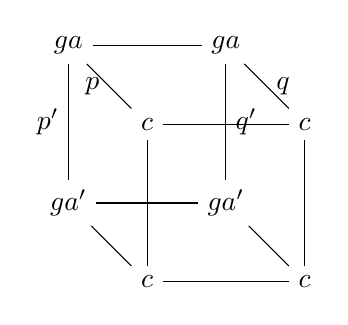
\begin{tikzpicture}
        \node (1) at (0,2) {\( ga \)};
        \node (2) at (2,2) {\( ga\)};
        \node (3) at (1,1) {\( c \)};
        \node (4) at (3,1) {\( c \)};
        \node (5) at (0,0) {\( ga' \)};
        \node (6) at (2,0) {\( ga' \)};
        \node (7) at (1,-1) {\( c \)};
        \node (8) at (3,-1) {\( c \)};
        \draw [-] (1) to node [] {} (2);
        \draw [-] (3) to node [] {} (4);
        \draw [-] (5) to node [] {} (6);
        \draw [-] (7) to node [] {} (8);
        \draw [-] (1) to node [left] {\( p \)} (3);
        \draw [-] (2) to node [right] {\( q \)} (4);
        \draw [-] (5) to node [] {} (7);
        \draw [-] (6) to node [] {} (8);
        \draw [-] (1) to node [left] {\( p' \)} (5);
        \draw [-] (2) to node [right] {\( q' \)} (6);
        \draw [-] (3) to node [] {} (7);
        \draw [-] (4) to node [] {} (8); 
      \end{tikzpicture}
    \]
    commutes and is filled because \( \C \) is a set. Therefore
    \(
         ( p,q ) = ( p',q' ) 
    \)
\end{proof}

\daniel{Is the lemma below sufficient?  It says the two codes are
  equivalent, but couldn't they still be empty?}

We now construct a point
\[
  \code ( \inr c , \ap_{\glue} a ) \tin
  \code ( \inr c , \inl fa ) =
  \code ( \inr c , \inl ga ).
\]
because both sides of the equality are propositions, a unique
definition for \( \code ( \inr c , \ap_{\glue} a ) \) exists if we
construct an equivalnce.

\begin{lemma} \label{thm:code-cfa-isequiv-code-cga}
  The functions
  \[
    \code ( \inr c , \inl fa ) \to \code ( \inr c , \inr ga ), \:
    ( p,q ) \mapsto p
  \]
  and
  \[
    \code ( \inr c , \inr ga ) \to \code ( \inr c , \inl fa ), \:
    r \mapsto ( r , \refl_{\inl fa} )
  \]
  form an equivalence. 
\end{lemma}
\begin{proof}
  First, let us show these actually are functions.
  
  Let
  \(
      ( p,q ) \tin \code ( \inr c , \inl fa ).
  \)
  since \( f \) is injective, we have that
  \(
      a =_\A a' .
  \)
  beta-reducing \( ga' \) to \( ga \), gives us that
  \(
      p \tin \code ( \inr c , \inr ga ).
  \)
  this provides the first
  function.

  Given
  \(
      r \tin \code ( \inr c , \inr ga ),
  \)
  \( r \) is equal to a
  point in
  \(
      c =_\C ga.
  \)
  this provides a point
  \(
      ( r , \refl_{fa} ) \tin \code ( \inr c , \inl fa ).
  \)
  this gives the second function.

  The functions form an equivalence because both
  \( \code ( \inr c , \inl fa ) \) and
  \( \code ( \inr c , \inr ga ) \) are propositions.
\end{proof}

% ~~~~~~~~~~~~~~~~~~~~~~~~~~~~~~

The next stage in proving theorem \ref{thm:pushout-is-set} is showing
that
\(
    \inl b =_{\BAC} x 
\)
and
\(
\inr c =_{\BAC} x
\)
are mere propositions for any \( x \).  To do so, we construct
equivalences between, respectively,
\(
    \code ( \inl b , x )
\)
and
\(
    \code ( \inr c , x )
\)
which we know are mere propositions. Specifically, we define maps
\begin{align*}
  \encode ( \inl b ) \from & \prod\limits_{x \tin \BAC}
    ( \inl b =_{\BAC} x ) \to \code ( \inl b , x ) \\
  \encode ( \inr c ) \from & \prod\limits_{x \tin \BAC}
    ( \inr c =_{\BAC} x ) \to \code ( \inr c , x ) \\
  \decode ( \inl b ) \from & \prod\limits_{x \tin \BAC}
    \code ( \inl b , x ) \to ( \inl b =_{\BAC} x ) \\
  \decode ( \inr c ) \from & \prod\limits_{x \tin \BAC}
    \code ( \inr c , x ) \to ( \inr c =_{\BAC} x ) \\
\end{align*}
with corresponding \( \encode \) and \( \decode \) pairs forming
mutual equivalences.

% ~~~~~~~~~~~~~~~~~~~~~~~~
% ~~~~~~~~~~~~~~~~~~~~~~~~

\subsection{defining \( \encode \)}
\label{sec:define-encode}

We define \( \encode ( \inl b ) \) and \( \encode ( \inr
c ) \) by inducting on \( x \tin \BAC \). In doing so, we make use of
path induction. 

Define 
\[
  \encode ( \inl (b) ) \from
  \prod\limits_{ x \tin \BAC } ( \inl (b) =_{\BAC} x ) \to
  \code (\inl(b) , x)
\] 
by the
% 
\(
    \refl_{\inl b} \mapsto \refl_{\inl' b}.
\)
% 
Recall, \( \inl \) corresponds to the pushout map into \( \BAC \)
and \( \inl' \) to the pushout map into
\( \code ( \inl b , \inl b' ) \).

Define 
\[
  \encode ( \inr c ) \from
  \prod\limits_{ x \tin \BAC } ( \inr c =_{\BAC} x ) \to
  \code ( \inr c , x)
\] 
by the assignemnt
\(
    \refl_{ \inr c} \mapsto \refl_c.
\)
Note, we use that
\(
    \code ( \inr c , \inr c )
\)
is equivalent to \( c =_\C c \) as shown in Lemma \ref{sec:code-cc-isprop}.

Define
\[
  \ap_{ \encode ( \inl b ) } \tin
  ( ( b =_{\BAC} fa ) \to \code ( \inl b , \inl fa ) ) =
  ( ( b =_{\BAC} ga ) \to \code ( \inl b , \inr ga ) )
\]
to be the diagram
\[
  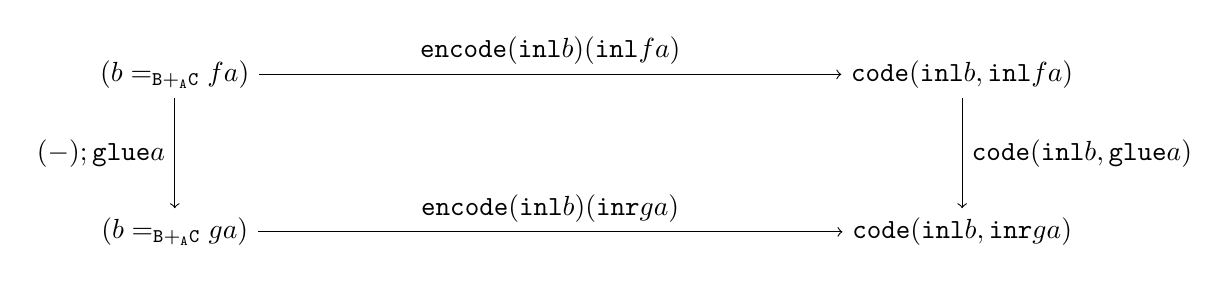
\begin{tikzpicture}
    \node (1) at (-5,1) {\( ( b =_{\BAC} fa ) \)};
    \node (2) at (-5,-1) {\( ( b =_{\BAC} ga ) \)};
    \node (3) at (5,1) {\( \code ( \inl b , \inl fa ) \)};
    \node (4) at (5,-1) {\( \code ( \inl b , \inr ga ) \)};
    \draw [->] (1) to node [left]
      {\( (-) ; \glue a \)} (2);
    \draw [->] (1) to node [above]
      {\( \encode ( \inl b ) ( \inl fa ) \)} (3);
    \draw [->] (2) to node [above]
      {\( \encode ( \inl b ) ( \inr ga ) \)} (4);
    \draw [->] (3) to node [right]
      {\( \code ( \inl b , \glue a ) \)} (4); 
  \end{tikzpicture}
\]
which commutes because \( \code ( \inl b , ga ) \) is a mere proposition.

Define
\[
  \ap_{ \encode ( \inr c ) } \tin
  ( ( c =_{\BAC} fa ) \to \code ( \inr c , \inl fa ) ) =
  ( ( c =_{\BAC} ga ) \to \code ( \inr c , \inr ga ) )
\]
to be the diagram
\[
  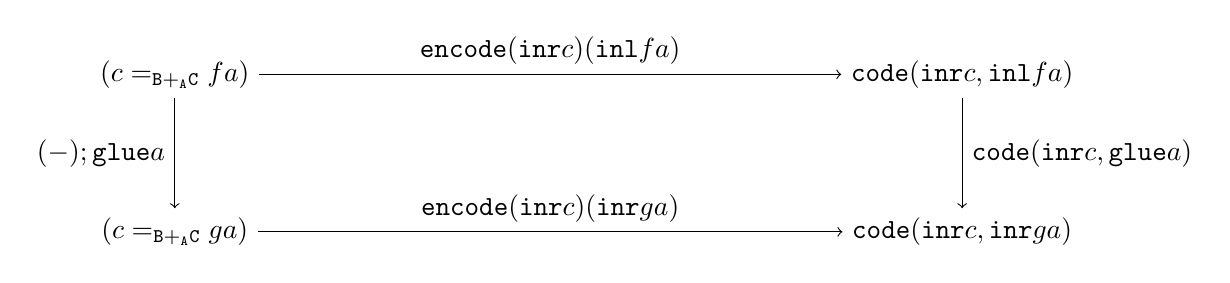
\begin{tikzpicture}
    \node (1) at (-5,1) {\( ( c =_{\BAC} fa ) \)};
    \node (2) at (-5,-1) {\( ( c =_{\BAC} ga ) \)};
    \node (3) at (5,1) {\( \code ( \inr c , \inl fa ) \)};
    \node (4) at (5,-1) {\( \code ( \inr c , \inr ga ) \)};
    \draw [->] (1) to node [left]
      {\( (-) ; \glue a \)} (2);
    \draw [->] (1) to node [above]
      {\( \encode ( \inr c ) ( \inl fa ) \)} (3);
    \draw [->] (2) to node [above]
      {\( \encode ( \inr c ) ( \inr ga ) \)} (4);
    \draw [->] (3) to node [right]
      {\( \code ( \inr c , \glue a ) \)} (4); 
  \end{tikzpicture}
\]
which commutes because \( \code ( \inr c , ga ) \) is a mere proposition.

% ~~~~~~~~~~~~~~~~~~~~
% ~~~~~~~~~~~~~~~~~~~~

\subsection{Defining \( \decode \)}
\label{sec:define-decode}

To define the map
\begin{equation} \label{eq:decode-b-blank}
  \decode ( \inl b ) \from
  \prod\limits_{x \tin \BAC} \code ( \inl b , x ) \to
  ( \inl b =_{\BAC} x )
\end{equation}
we use induction on \( x \tin \BAC \) which, in practice, means that
we need two function types
\begin{itemize}
\item
  \(
    \decode ( \inl b ) ( \inl b' ) \from
    \code (\inl b , \inl b') \to
    ( \inl b =_{\BAC} \inl b' )
  \)
\item
  \(
    \decode ( \inl b ) ( \inr c ) \from
    \code ( \inl b , \inr c ) \to
    ( \inl b =_{\BAC} \inr c
  \) 
\end{itemize}
and a witness
\begin{align*}
  \ap_{\decode ( \inl b )} (\glue a) &
  \tin
  ( \code ( \inl b , \inl fa ) \to ( \inl b =_{\BAC} \inl fa ) \\
  & =
  ( \code ( \inl b , \inr ga ) \to ( \inl b =_{\BAC} \inr ga )
\end{align*}

% ~~~~~~~~~~~~~~~~~~

Define
\[
  \decode ( \inl b ) \from
  \code ( \inl b , \inl b' ) \to
  ( \inl b =_{\BAC} \inl b' )
\]
by inducting on
\(
    \code ( \inl b , \inl b' )
\)
This requires three values.
\begin{itemize}
\item
  Let
  \(
    \decode ( \inl b) ( \inl b' ) (\inl' p)
    \tin ( \inl b =_{\BAC} \inl b' ),
  \)
  where
  \(
    p \tin b =_{\B} b',
  \)
  be
  \(
    \ap_{\inl} (p);
  \)
\item
  Let
  \(
    \decode (\inl b ) ( \inr c ) ( \inr' (q,r,s) ) \tin ( b ={\BAC} b' ),
  \)
  where
  \(
    (q,r,s) \tin
    \sum\limits_{a,a' \tin \A}
    ( b =_\B fa ) \times (b' =_\B fa' ) \times ( ga =_\C ga' ),
  \)  
  be
  \(
    ap_{\inl} q ; \glue a ; \ap_{\inr} s ; \glue^{-1} a' ; r^{-1}
  \)
  and
\item
  The path
  \begin{align*}
    \ap_{\decode ( \inl b )} ( \glue (t,u,v) )
    & \tin ( \decode ( \inl b )
      ( \inl' ( \alpha (t,u,v) ) ) =_{\inl b =_{\BAC} \inl b'} \\
    & \decode ( \inl b ) ( \inr' ( \beta (t,u,v) ) ),
  \end{align*}
  where
  \(
    (t,u,v) \tin
    ( b =_\B fa ) \times ( b' =_\B fa' ) \times ( b =_\B b' ),
  \)
  is trivial because
  \(
    \code ( \inl b , \inl b' )
  \)
  is a mere set.
\end{itemize}

% ~~~~~~~~~~~~~~~~~~ 

To define
\[
  \decode ( \inl b ) \from
  \code ( \inl b , \inr c ) \to
  ( \inl b =_{\BAC} \inr c ),
\]
recall that
\[
  \code ( \inl b , \inr c ) =
  \sum\limits_{a \tin \A} (b =_{\B} fa) \times (c =_{\C} ga)
\]
Define
\[
  \decode ( \inl b ) ( p , q ) \coloneqq
  \inl p ; \glue a ; \inr q
\]

% ~~~~~~~~~~~~~~~~~~ 

Right now, we define
\begin{align*}
  \ap_{\decode ( \inl b ) } (\glue a) & \tin
  ( \code ( \inl b , \inl fa ) \to ( \inl b =_{\BAC} \inl fa ) \\
  & =
  ( \code ( \inl b , \inl ga ) \to ( \inl b =_{\BAC} \inl ga )
\end{align*}
To define this is to construct a commuting square
\[
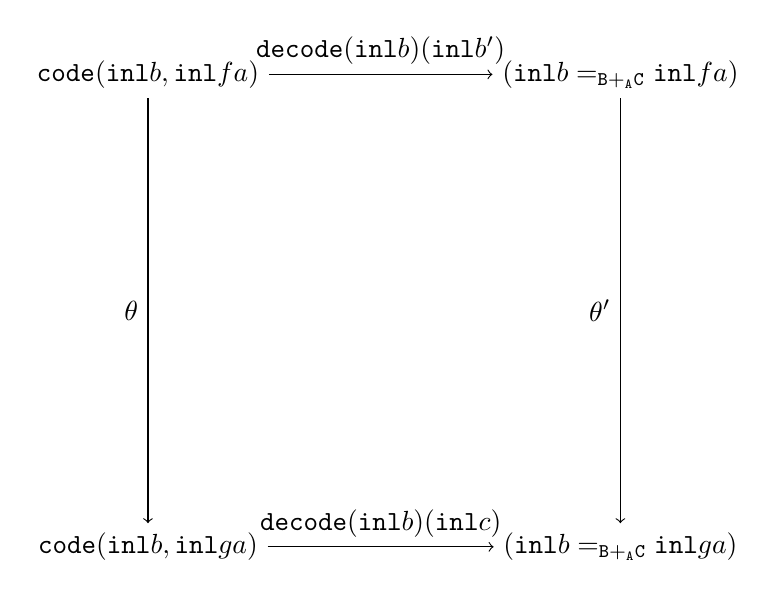
\begin{tikzpicture}
  \node (1) at (-3,3)
    {\( \code ( \inl b , \inl fa ) \)};
  \node (2) at (-3,-3)
    {\( \code ( \inl b , \inl ga ) \)};
  \node (3) at (3,3)
    {\( ( \inl b =_{\BAC} \inl fa ) \)};
  \node (4) at (3,-3)
    {\( ( \inl b =_{\BAC} \inl ga ) \)};
  \draw [->] (1) to node [left]
    {\( \theta \)} (2);
  \draw [->] (1) to node [above]
    {\( \decode (\inl b )(\inl b') \)} (3);
  \draw [->] (3) to node [left]
    {\( \theta' \)} (4);
  \draw [->] (2) to node [above]
    {\( \decode (\inl b )(\inl c) \)} (4);
\end{tikzpicture}
\]
We have already defined the two \( \decode \) maps. The map \( \theta'
\) is post-composition by \( \glue a \). The map \( \theta \) requires
induction to define because we are mapping out of a pushout.
Therefore, we need the following three values to define \( \theta \):
\begin{itemize}
\item
  \(
    \theta (\inl' p)
  \)
  for
  \(
    p \tin b =_\B fa
  \)
\item
  \(
    \theta ( \inr' (q,r,s) )
  \)
  for
  \(
    (q,r,s) \tin
      \sum\limits_{a',a'' \tin \A}
      (b=_\B fa') \times (fa =_B fa'') \times (ga' =_C ga'')
  \) 
\item
  \(
    \ap_{ \theta } ( \glue (t,u,v) ) \tin
      \theta ( \inl' (\alpha (t,u,v) ) ) =
      \theta ( \inr' ( \beta (t,u,v) ) )
  \).
\end{itemize}

A quick remark on notation: since \( f \) is monic and \( \B \) is a
set, we can pull back any path of form \( r \tin fa =_\B fa'\) to a
determined path
\(
  \hat{r} \tin a =_\A a'.
\)

Define
\(
  \theta (\inl' p)
\)
for
\(
  p \tin b=_\B fa
\)
to be
\(
  ( p , \refl_{ga} ).
\)
Define
\(
  \theta ( q,r,s )
\)
to be
\(
  ( q , \ap_g ( \hat{r} ) ; s^{-1} ).
\)

Now we know that
\(
  \ap_{ \theta } ( \glue ( t,u,v ) )
\)
is a path from
\(
  \theta ( \inl' ( v ) ) = ( v , \refl_{ga} )
\)
to
\(
  \theta ( \inr' ( \beta ( t,u,v ) ) )
\)
But that can be reduced:
\begin{align*}
  \theta ( \inr' ( t,u,\ap_{g}(\hat{v}) ) )
  & = ( t, \ap_g ( \hat{u} ); \ap_g ( \hat{v} )^{-1} ) \\
  & = ( t, \ap_g ( \hat{u} ; \hat{v}^{-1}) ).
\end{align*}
With this in mind, we define
\(
  \ap_{\theta} ( \glue ( t,u,v ) )
\)
to be post-composition by
\[
  ( \ap_f ( \hat{u};\hat{v}^{-1} ) , \ap_g ( \hat{u};\hat{v}^{-1} ) ).
\]

Now we need to check that the diagram commutes.  Since
\(
  \code ( \inl b , \inl fa )
\)
is a set, it suffices to check that
\[
  \theta' ( \decode (\inl b ) ( \inl fa ) ( x ) )
    =_{ \inl b =_{\BAC} \inr ga }
    \decode ( \inl b )(\inr ga) ( \theta ( x ) )
\]
where
\(
  x \tin \code ( \inl b, \inl fa )
\)
takes values
\begin{itemize}
\item
  \(
    \inl' p
  \)
  for
  \(
    p \tin b=_\B fa,
  \)
  and
\item
  \(
    \inr' ( q,r,s )
  \)
  for
  \(
    ( q,r,s ) \tin
      \sum\limits_{a',a'' \tin \A}
      (b=_\B fa') \times ( fa =_\B fa'' )\times ( ga'=_\C ga'' ).
  \)
\end{itemize}
We also need to check that
\[
  \ap_{ \theta' ; \decode ( \inl b ) ( \inl fa ) )} ( \glue ( t,u,v ) ) 
    =_{ \inl b =_{\BAC} \inr ga }
    \ap_{ \decode ( \inl b )(\inr ga) ; \theta } ( \glue ( t,u,v ) ) 
\]

Set
\(
  x \coloneqq \inl' p.
\)
Then
\begin{align*}
  \theta' ( \decode ( \inl b ) ( \inl fa ) ( \inl' p ) )
  & = \theta' ( ( \ap_{\inl'} p ) ) \\
  & = \ap_{\inl'} p ; \glue a
\end{align*}
Also,
\begin{align*}
  \decode ( \inl b ) ( \inr ga ) ( \theta ( \inl' p ) )
  & = \decode ( \inl b ) ( \inr ga ) ( ( p,\refl_{ga} ) ) \\
  & = \ap_{\inl'} p ; \glue a ; \ap_{\inr'} \refl_{ga} \\
  & = \ap_{\inl'} p ; \glue a ; \refl_{\inr' ga} \\
  & = \ap_{\inl'} p ; \glue a
\end{align*}
Therefore, the square commutes on \( \inl' p \)

Set
\(
  x \coloneqq \inr' ( q,r,s ).
\)
Then
\begin{align*}
  \theta' ( \decode ( \inl b ) ( \inl fa ) ( \inr' ( q,r,s ) ) )
  & = \theta' ( \ap_{\inl} q ; \glue a' ; \ap_{\inr} s ; \glue a'' ;
    \ap_{\inl} r^{-1} ) \\
  & =  \ap_{\inl} q ; \glue a' ; \ap_{\inr} s ; \glue^{-1} a'' ;
    \ap_{\inl} r^{-1} ; \glue a \\
   & =  \ap_{\inl} q ; \glue a' ; \ap_{\inr} s ; \glue^{-1} a'' ;
    \ap_{\inl} \ap_f \hat{r}^{-1} ; \glue a \\
\end{align*}
Also,
\begin{align*}
  \decode ( \inl b ) ( \inr ga ) ( \theta ( \inr' ( q,r,s ) ) )
  & = \decode ( \inl b )( \inr ga )( q , \ap_g ( \hat{r} ; s^{-1}
    ) ) \\
  & = \ap_{\inl} q ; \glue a' ; ( \ap_{\inr} ( \ap_g \hat{r} ; s^{-1} )^{-1} ) \\
  & = \ap_{\inl} q ; \glue a' ; \ap_{\inr} ( \ap_g ( \hat{r} ) ; ( \ap_g
    (s^{-1}) )^{-1} ) \\
  & = \ap_{\inl} q ; \glue a' ; \ap_{\inr} (s^{-1})^{-1} ;  \ap_g ( \hat{r} )^{-1} \\
  & = \ap_{\inl} q ; \glue a' ; \ap_{\inr} (s^{-1})^{-1} ;  \ap_g ( \hat{r} )^{-1} \\
  & = \ap_{\inl} q ; \glue a' ; \ap_{\inr} s ;  \ap_g ( \hat{r} )^{-1} \\
\end{align*}
We just need to check that
\[
  \ap_g ( \hat{r} )\inv =
  \glue\inv a'' ; \ap_{ \inl } \ap_f \hat{r}\inv ; \glue a
\]
But this follows from the continuity of \( \glue \), that is, it
preserves paths. Therefore, the square commutes on
\(
  \inr' ( q,r,s ).
\)

It remains to check that
\[
  \ap_{\theta' ; \decode (\inl b ) ( \inl fa ) )} ( \glue ( t,u,v ) ) 
  =_{ \inl b =_{\BAC} \inr ga }
  \ap_{ \decode ( \inl b )(\inr ga) ; \theta } ( \glue ( t,u,v ) ) 
\]
for
\(
  ( t,u,v ) \tin
  \sum\limits_{a',a''\tin \A}
  ( b =_\B fa' ) \times ( fa =_\B fa'' ) \times ( b =_{\B} fa ).
\)
Here, we make some reductions.
\begin{itemize}
\item
  Because \( f \) is monic, we get that
  \(
    fa =_\B fa''
  \)
  reduces to
  \(
    fa =_\B fa.
  \)
  Since \( \B \) is a set, we can take
  \(
    u = \refl_{fa}.
  \)
\item
  The type
  \(
    b =_\B fa'
  \)
  reduces to
  \(
    fa =_\B fa
  \)
  because \( \B \)
  is monic, so
  \(
    t = \refl_{fa}.
  \).
\item
  The type
  \(
    b =_\B fa
  \)
  reduces to
  \(
    fa =_\B fa
  \)
  because \( \B \) is monic, so
  \(
    v = \refl_{fa}.
  \)
\end{itemize}
Without loss of generality, we can take
\(
  ( t,u,v ) = ( \refl_{fa},\refl_{fa},\refl_{fa} ).
\)
Therefore, it suffices to check that 
\begin{align*}
   & \ap_{\theta' ; \decode (\inl b ) ( \inl fa ) )}
   ( \glue ( \refl_{fa},\refl_{fa},\refl_{fa} ) ) \\
        & =_{ \inl b =_{\BAC} \inr ga }
        \ap_{ \decode ( \inl b )( \inr ga ) ; \theta }
        ( \glue  ( \refl_{fa},\refl_{fa},\refl_{fa} ) ). 
\end{align*}
  
But because the square commutes on points as shown above, the two
paths on the left and right of the above equation are certainly
parallel.  Then functorality gives us that \( \refl_{fa} \) is
preserved. Hence the square commutes.

% ~~~~~~~~~~~~~~~~~~~

To define the map
\[
  \decode ( \inr c ) \from
  \prod\limits_{x \tin \BAC}
  \code ( \inr c , x ) \to \inr ( c =_{\BAC} x )
\]
we use induction on \( \BAC \) which, in practice, means that we
require the two function types
\begin{itemize}
\item
  \(
    \decode ( \inr c ) ( \inl b ) \from
      \code (\inr c , \inl b) \to
      ( \inr c =_{\BAC} \inl b )
  \)
\item
  \(
    \decode ( \inr c ) ( \inr c' ) \from
      \code ( \inr c , \inr c' ) \to
      ( \inr c =_{\BAC} \inr c' )
  \) 
\end{itemize}
and a witness
\begin{align*}
  \ap_{\decode ( \inr c ) } (\glue a) & \tin
  ( \code ( \inr c , \inl fa ) \to ( \inr c =_{\BAC} \inl fa ) \\
  & = ( \code ( \inr c , \inl ga ) \to ( \inr c =_{\BAC} \inl ga )
\end{align*}

% ~~~~~~~~~~~~~~~~~~~~``

First, let us define the map
\[
  \decode ( \inr c ) ( \inl b ) \from
    \code ( \inr c , \inl b ) \to
    ( \inr c =_{\BAC} \inl b ).
\]
Recall that
\(
  \code ( \inr c , \inl b ) \coloneqq
    \sum\limits_{a \tin \A}
    ( c =_{\C} ga ) \times ( b =_{\B} fa ).
\)
Thus for any \( ( p,q ) \) in
\(
  \code ( \inr c , \inl b ),
\)
we define a path
\(
  \decode ( \inr c ) ( \inl b ) ( p,q )
\)
in \( \BAC \) from \( \inr c \) to  \( \inl b \). Take this path to be
\(
  \inr p ; \glue^{-1}  a ; \inl q^{-1}.
\)

% ~~~~~~~~~~~~~~~~~

Next, we define
\[
  \decode ( \inr c ) ( \inr c' ) \from
  \code ( \inr c , \inr c' ) \to
  ( \inr c =_{\BAC} \inr c' ).
\]
Recall that
\[
  \code ( \inr c , \inr c' ) \coloneqq
  \sum\limits_{a \tin \A}
  ( c =_{\C} ga ) \times ( c' =_{\C} ga' ) \times ( fa =_{\B} fa' ). 
\]
Thus for any \( ( p,q,r ) \) in
\(
  \code ( \inr c , \inr c' ),
\)
we define a path
\(
  \decode ( \inr c ) ( \inr c' ) ( p,q,r )
\)
in \( \BAC \) from \( \inr c \) to \( \inr c' \). Take this path to be
\(
  \inr p ; \glue\inv a ; \inl r \glue a' ; \inr q\inv.
\)

% ~~~~~~~~~~~~~~~~~~

Finally, we define a path
\begin{align*}
  \ap_{\decode ( \inr c )} (\glue a) & \tin
  ( \code ( \inr c , \inl fa ) \to ( \inr c =_{\BAC} \inl fa ) \\
  & =  ( \code ( \inr c , \inl ga ) \to ( \inr c =_{\BAC} \inl ga ).
\end{align*}
Replacing the two \( \code \) expressions with their definitions, this
path is constructed as a commuting square
\[
  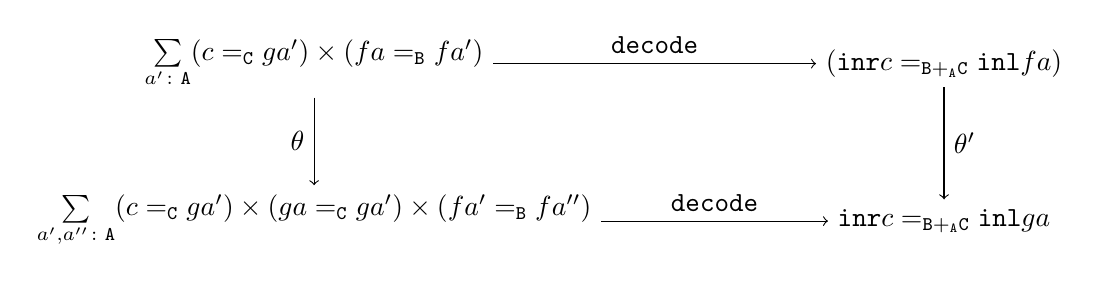
\begin{tikzpicture}
    \node (1) at (-4,1)
      { \(
        \sum\limits_{a' \tin \A}
        ( c =_{\C} ga' ) \times ( fa =_{\B} fa' )
      \) }; 
    \node (2) at (-4,-1)
      { \(
        \sum\limits_{a',a'' \tin \A}
        ( c =_{\C} ga' ) \times ( ga =_{\C} ga' ) \times
        ( fa' =_{\B} fa'' )
      \) };
    \node (3) at (4,1)
      { \(
        ( \inr c =_{\BAC} \inl fa )
      \) };
    \node (4) at (4,-1)
      { \(
        \inr c =_{\BAC} \inl ga
      \) };
    \draw [->] (1) to node [left] {\( \theta \)} (2);
    \draw [->] (1) to node [above] {\( \decode \)} (3);
    \draw [->] (2) to node [above] {\( \decode \)} (4);
    \draw [->] (3) to node [right] {\( \theta' \)} (4); 
  \end{tikzpicture}
\]
The easier map to define is \( \theta' \) which  concatenates
with \( \glue a \).  Then \( \theta \) is given by
\(
  ( p,q ) \mapsto ( p, \refl_{ga} , q ).
\)
Now we check whether the square commutes. We have
\begin{align*}
  \theta' ( \decode ( \inr c , - ) ( \inl fa ) ( p,q ) )
  & = \theta' ( \inr p ; \glue^{-1} a' ; \inl q^{-1}  ) \\
  & = \inr p ; \glue^{-1} a' ; \inl q^{-1} ; \glue a. \\
\end{align*}
We also have that
\begin{align*}
  \decode ( \inr c , - ) ( \inl ga ) ( \theta ( p,q ) )
  & = \decode ( \inr c , - ) ( \inl ga ) ( p,\refl_{ga},q ) \\
  & =  \inr p ; \glue\inv a' ; \inl q\inv ; \glue a ; \inr \refl_{ga} \\
  & =  \inr p ; \glue\inv a' ; \inl q\inv ; \glue a  \\
\end{align*}
Hence the square commutes.

% ~~~~~~~~~~~~~~~~~~~~~~~~
% ~~~~~~~~~~~~~~~~~~~~~~~~

\subsection{Composing encode and decode}

Consider the composite
\[
  \encode ; \decode
  \from
  \prod\limits_{x,y \tin \BAC} x =_{\BAC} y
  x =_{\BAC} y
\]
To show that this map is the identity up to homotopy, we compute both
\begin{itemize}
\item
  \(
    \encode ; \decode ( \inl b ) \from
      \prod\limits_{x \tin \BAC}
      ( \inl b =_{\BAC} x ) \to ( \inl b =_{\BAC} x ),
   \)
   and
\item
  \(
    \encode ; \decode ( \inr c  ) \from
      \prod\limits_{x \tin \BAC}
      \inr c =_{\BAC} x \to ( \inr c =_{\BAC} x ).
  \)
\end{itemize}
But computing these values actually requires the computation of the
following four maps:
\begin{itemize}
\item
  \(
    \encode ; \decode ( \inl b )(\inl b') \from
      \code ( \inl b , \inl b' ) \to
      ( \inl b =_{\BAC} \inl b' ).
  \)
  By path induction, it suffices to check \( \refl_{\inl b} \):
  \begin{align*}
    \encode ; \decode ( \inl b )(\inl b') ( \refl_{\inl b} ) & =
    \encode ( \ap_{\inl'} \refl_{\inl b} ) \\ & =
    \encode (\refl_{\inl' b} ) \\ & =
    \ap_{\inl} \refl_{\inl' b} \\ & =
    \refl_{\inl b}.
  \end{align*}
  So this one checks out.
\item
  \(
    \encode ; \decode ( \inl b ) (\inr c) \from
      \code ( \inl b , \inr c ) \to
      ( \inl b =_{\BAC} \inl c ).
  \)
  \daniel{glue(a) *is* the only thing to check here, right?}
  This is only non-trivial when
  \(
    b =_\B fa
  \)
  and
  \(
    c =_\C ga.
  \)
  Hence
  \[
    \encode ; \decode ( \inl b ) ( \inr c ) ( \glue a ) =
    \decode ( \inl b ) ( \inr c ) ( \refl_{fa} , \refl_{ga} ) =
    \ap_{\inr} \refl_{ga} ; \glue a ; \ap_{\inl} \refl_{fa} =
    \glue a.
  \]
  This one checks out too.
\item
  \(
    \encode ; \decode ( \inr c , - )(\inl b) \from
    \code ( \inr c , \inl b ) \to ( \inr c =_{\BAC} \inl b ).
  \)
  This is symmetric to the above case, so checks out. 
\item
  \(
  \encode ; \decode ( \inr c , - )(\inr c') \from
  \code ( \inr c, \inr c' ) \to
  ( \inr c =_{\BAC} \inr c' )
  \)
  is, by path induction, 
  \[
    \encode ; \decode ( \inr c , - )(\inr c') ( \refl_{\inr c} ) =
    \decode ( \inr c , - )(\inr c') ( \refl_c ) =
    \ap_{\inr} \refl_c =
    \refl_{\inr c}
  \]  
\end{itemize}

And so, we have proved that \( \decode \) is a section for \( \encode
\). The opposite direction remains.

% ~~~~~~~~~~~~~~~~~~

Now, we look at the composite
\[
  \decode ; \encode \from
  \prod\limits_{x,y \tin \BAC} \code ( x,y ) \to
  \code ( x,y )
\]
We can compute this composite by computing the values
\begin{itemize}
\item
  \(
    \decode ; \encode (\inl b ) ( \inl b' ) \from
    \code ( \inl b , \inl b' ) \to
    \code ( \inl b , \inl b' ),
  \)
\item
  \(
    \decode ; \encode (\inl b ) ( \inr c ) \from
    \code ( \inl b , \inr c ) \to
    \code ( \inl b , \inr c ),
  \)
\item
  \(
    \decode ; \encode (\inr c ) ( \inl b ) \from
    \code ( \inr c , \inl b ) \to
    \code ( \inr c , \inl b ),
    \)
  and  
\item
  \(
    \decode ; \encode (\inr c ) ( \inr c' ) \from
    \code ( \inr c , \inr c' ) \to
    \code ( \inr c , \inr c' )
  \)
\end{itemize}
But these maps are all identity since \( \code (x,y) \) is a
proposition for \( x , y \tin \BAC \).   

% ~~~~~~~~~~~~~~~~~~

We now know that
\(
    \encode
\)
and
\(
    \decode
\)
are mutual inverses. Therefore,
\(
    \inl b =_{ \BAC  } x
\)
and
\(
    \inr c =_{ \BAC } x
\)
are mere propositions for any
\(
    x \tin \BAC.
\)
As discussed above, the embedding
\(
    \P \hookrightarrow \Q
\)
is actually an equivlance. Theorem \ref{thm:pushout-is-set} follows.


%%%%%%%%%%%%%
% end document
%%%%%%%%%%%%%

\end{document}
